% !TEX root = x-sec-pruebas-penetracion-mas-rapidas.tex

\documentclass{beamer}
% \usetheme{Copenhagen}
\usecolortheme{beaver}
\setbeamercolor{block body alerted}{bg=alerted text.fg!10}
\setbeamercolor{block title alerted}{bg=alerted text.fg!20}
\setbeamercolor{block body}{bg=structure!10}
\setbeamercolor{block title}{bg=structure!20}
\setbeamercolor{block body example}{bg=green!10}
\setbeamercolor{block title example}{bg=green!20}
\usepackage{tikz}   
\usepackage[utf8]{inputenc}
\usepackage[spanish]{babel}

\usepackage{hyperref}
\hypersetup{
    colorlinks=true,
    linkcolor=blue,
    filecolor=magenta,      
    urlcolor=cyan,
}

\usepackage{dirtytalk}

\title{Pruebas de penetración mas rápidas mediante el uso de herramientas de código libre}
\author{Santiago Lizardo}
\date{16 de Junio de 2025}

\begin{document}

\begin{frame}
	\begin{center}
		
\includegraphics[width=0.3\textwidth]{images/xsec_logo.jpeg}
	\end{center}

	\maketitle
\end{frame}

\begin{frame}
	\frametitle{Sobre mi}

	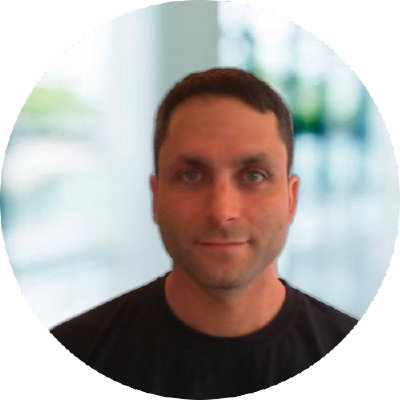
\includegraphics[width=0.4\textwidth]{images/santiago-lizardo.png}

	\begin{itemize}
		\item Mas de 20 años en el mundo de software
		\item Entusiasta de la seguridad informática
		\item Fundador de Reconmap
		\item \url{https://github.com/santiagolizardo}
		\item \url{https://www.linkedin.com/in/santiagolizardo/}
	\end{itemize}
\end{frame}

\begin{frame}
	\frametitle{Lo parte divertida de ciberseguridad}
	Buscar y explotar vulnerabilidades.
\end{frame}

\begin{frame}
	\frametitle{Escalando el trabajo}
	De una tarea y cliente, a varios clientes y proyectos.
\end{frame}

\begin{frame}
	\frametitle{La parte menos divertida}
	Generar reportes, ejecutar los mismos comandos una y otra vez.
\end{frame}

\begin{frame}
	\frametitle{La idea detras de DRY}
	Explicación del principio DRY (Don't Repeat Yourself).
\end{frame}

\begin{frame}
	\frametitle{Scripting y templating de comandos para ahorrar tiempo}
	Uso de scripts y plantillas para automatizar tareas repetitivas.
\end{frame}

\begin{frame}
	\frametitle{Templating de reportes}
	Automatización de la generación de reportes.
\end{frame}

\begin{frame}
	\frametitle{Herramientas disponibles de código libre}
	Revisión de herramientas open source útiles para pentesting.
\end{frame}

\begin{frame}
	\frametitle{Introducción a Reconmap}
	Presentación de la plataforma Reconmap.
\end{frame}

\begin{frame}
	\frametitle{Misión}
	Objetivo principal de Reconmap.
\end{frame}

\begin{frame}
	\frametitle{Para quien está diseñado}
	Público objetivo de Reconmap.
\end{frame}

\begin{frame}
	\frametitle{Historia de Reconmap}
	Breve historia y evolución del proyecto.
\end{frame}

\begin{frame}
	\frametitle{Funcionalidades}
	Principales características y funcionalidades de Reconmap.
\end{frame}

\begin{frame}
	\frametitle{Arquitectura}
	Descripción de la arquitectura de Reconmap.
\end{frame}

\begin{frame}
	\frametitle{Pasos para tenerlo funcionando}
	Guía rápida para poner en marcha Reconmap.
\end{frame}

\begin{frame}
	\frametitle{Demostración en vivo}
	Presentación práctica de Reconmap en funcionamiento.
\end{frame}

\begin{frame}
	\frametitle{Ideas para el futuro}
	Propuestas y planes para el desarrollo futuro de Reconmap.
\end{frame}

\begin{frame}
	\frametitle{Llamado a la acción}
	Invitación a participar y contribuir al proyecto.
\end{frame}


\begin{frame}
	\frametitle{Architecture}

	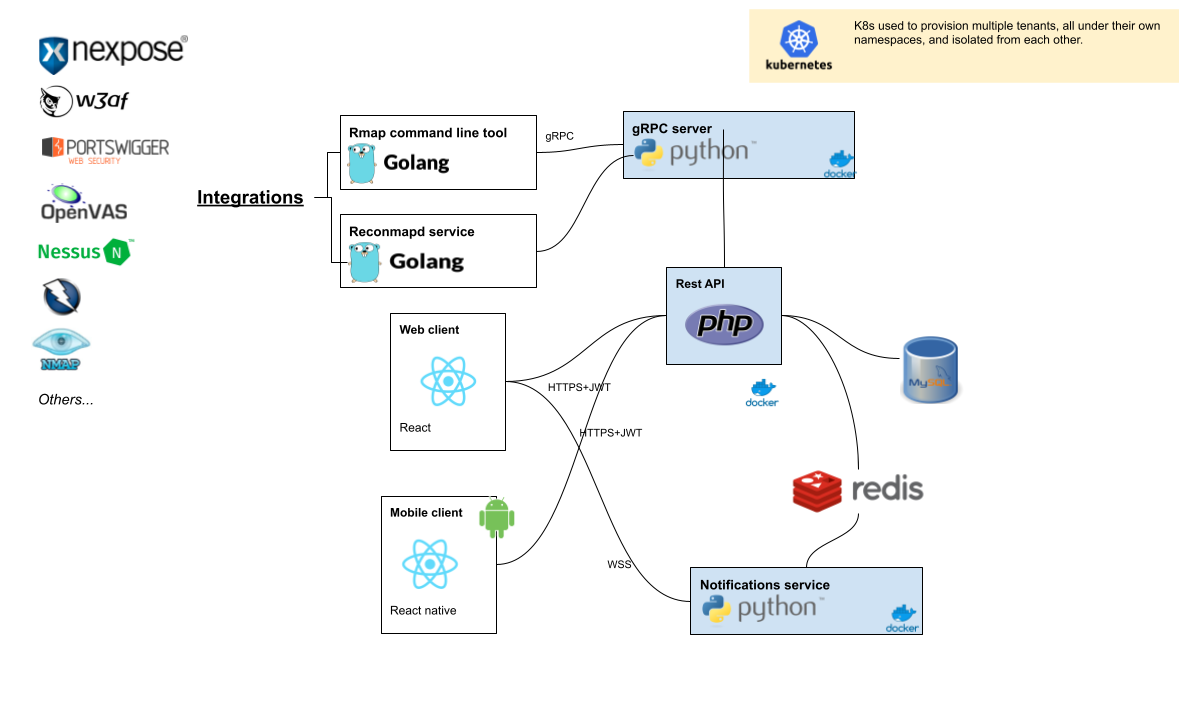
\includegraphics[width=\textwidth]{images/reconmap-architecture.png}
\end{frame}

\section{Staying in touch}

\begin{frame}{Staying in touch}
	
\includegraphics[width=0.4\textwidth]{images/reconmap-logo.png}
	\begin{itemize}
		\item \href{https://github.com/reconmap}{https://github.com/reconmap}
		\item \href{https://gitter.im/reconmap/community}{Gitter} chat
	\end{itemize}
	\bigskip

	
\includegraphics[width=0.2\textwidth]{images/xsec_logo.jpeg}
	\begin{itemize}
		\item \url{https://x-sec.sh}
	\end{itemize}
\end{frame}

\end{document}

